% !TeX program = xelatex

\documentclass[aspectratio=169]{beamer}
\usepackage{minted}
\usepackage{xcolor}
\usepackage{tcolorbox}
\usepackage{graphicx}
\usepackage{fontspec}
\usepackage{pifont}
\usepackage{hyperref}

\usetheme{default}
\setbeamertemplate{footline}[frame number]
\setbeamertemplate{navigation symbols}{}

\BeforeBeginEnvironment{minted}{\begin{tcolorbox}}
\AfterEndEnvironment{minted}{\end{tcolorbox}}

\AtBeginSection{
    \begin{frame}{Outline}
        \tableofcontents[currentsection, hideothersubsections]
    \end{frame}
}

\AtBeginSubsection{
    \begin{frame}{Outline}
        \tableofcontents[currentsection, currentsubsection]
    \end{frame}
}

\hypersetup{
    colorlinks=true,
    linkcolor=blue,
    urlcolor=cyan
}

\graphicspath{{../../images/}}



% Item style

\setbeamertemplate{itemize item}{\ding{108}}

% Block style

\setbeamercolor{block body alerted}{fg=white,bg=red}
\setbeamercolor{block body standard}{fg=black,bg=white}
\setbeamertemplate{blocks}[rounded][shadow=false]

% Alias for highlight text in orange and bold
\newcommand{\highlight}[1]{\textcolor{orange}{\textbf{#1}}}

% Command for captions
\renewcommand{\caption}[1]{%
    \begin{center}
        \scriptsize #1
    \end{center}%
}

%Information to be included in the title page:
\title{Kokkos and performance portability: an introduction for all}
\author{Mathieu Lobet and the CExA team}
\institute{CEA}
\date{2024}

% _____________________________________________________________________________

\begin{document}

\begin{frame}{}
    \titlepage
    \begin{center}
        \includegraphics[width=0.15\textwidth]{kokkos.png}%
        \hspace{2em}%
        \includegraphics[width=0.15\textwidth]{cexa_logo.png}
    \end{center}
\end{frame}

% _____________________________________________________________________________

\begin{frame}{This course is open source}
    \begin{center}
        \includegraphics[width=0.3\textwidth]{GitHub-logo.png}

        \href{https://github.com/CExA-project/cexa-kokkos-tutorials}{https://github.com/CExA-project/cexa-kokkos-tutorials}
    \end{center}
\end{frame}

% _____________________________________________________________________________

\begin{frame}{Prerequisites}
    This course is intended for beginners in Kokkos and performance portability without strong C++ knowledge

    \begin{itemize}
        \item Basic knowledge of C/C++
        \item Basic knowledge of parallel programming
        \item Basic knowledge of CMake
        \item Basic knowledge of a Linux environment
    \end{itemize}
\end{frame}

% _____________________________________________________________________________

\begin{frame}{Duration of the course}
    \begin{itemize}
        \item Course + practical work: full day
        \item Course + corrected exercise: half day
        \item Short version: 3 hours
    \end{itemize}
\end{frame}

\begin{frame}{Outline}
    \tableofcontents[hidesubsections]
\end{frame}

% _____________________________________________________________________________

\section{Introduction}

% _____________________________________________________________________________

\begin{frame}{Presentation of CExA}
    \begin{center}
        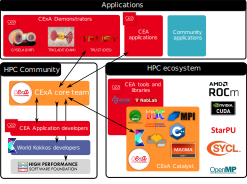
\includegraphics[width=0.7\textwidth]{cexa.png}
    \end{center}
\end{frame}

% _____________________________________________________________________________

\begin{frame}{Current supercomputers use a wide variety of hardware technologies}
    \begin{center}
        \includegraphics[width=1\textwidth]{top10_super_computers.png}

        \caption{Top 10 supercomputers in the world in June 2024}
    \end{center}

    \begin{itemize}
    \item Heterogeneous nodes: mix of CPU and GPU accelerators
    \item Many CPU (Intel, AMD, ARM, RISC) and GPU vendors (NVIDIA, AMD, Intel)
    \end{itemize}
\end{frame}

% _____________________________________________________________________________

\begin{frame}{EuroHPC supercomputers}
    \begin{center}
        \includegraphics[width=1\textwidth]{euroHPC.png}

        \caption{EuroHPC supercomputers}
    \end{center}
\end{frame}

% _____________________________________________________________________________

\begin{frame}{French national academic supercomputers}
    \begin{center}
    \includegraphics[width=0.8\textwidth]{french_super_computers.png}

    \caption{French academic and CEA supercomputers}
    \end{center}
\end{frame}

% _____________________________________________________________________________

\begin{frame}{Top500 GPU-CPU system share}
    \begin{center}
        \includegraphics[width=0.9\textwidth]{top500_cpu_gpu_share_history.png}
    \end{center}

    \structure{Note:} Does not include exotic and Intel Knight Landing accelerators
\end{frame}

% _____________________________________________________________________________

\begin{frame}{Basic definition of a supercomputer}
    \begin{itemize}
        \item A supercomputer is a distributed memory system composed of many compute nodes packed into racks and linked by a high-speed network
        \item Compute nodes are composed of one or more CPUs and one or more accelerators
        \item Most common accelerators today are GPGPU for General Purpose Graphic Processing Units
    \end{itemize}
    \begin{center}
        \includegraphics[width=\textwidth]{super-computer_architecture.png}
    \end{center}
\end{frame}

% _____________________________________________________________________________

\begin{frame}{Zoom on the CPU architecture}
    \begin{itemize}
        \item CPUs are designed for general purpose, from sequential task to parallel computing. They run the operating system as well
        \item Tens to hundred of cores in biggest processors
        \item SIMD (Single Instruction Multiple Data) units for accelerating arithmetic operations
    \end{itemize}
    \begin{center}
        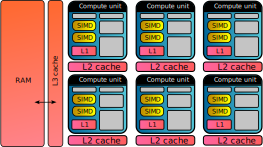
\includegraphics[width=0.6\textwidth]{cpu_architecture.png}
    \end{center}
\end{frame}


% _____________________________________________________________________________

\begin{frame}{Zoom on the GPU architecture}
    \begin{itemize}
        \item GPUs are designed to achieve massive parallelism of simple kernels
        \item Hundreds of computing units, thousands of threads
        \item Large SIMT vector unit (Single Instruction Multiple Threads) per computing unit
    \end{itemize}
    \begin{center}
        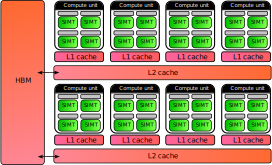
\includegraphics[width=0.6\textwidth]{gpu_architecture.png}
    \end{center}
\end{frame}

% _____________________________________________________________________________

\begin{frame}{Main difference between CPU and GPU}
    \begin{center}
        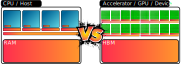
\includegraphics[width=0.8\textwidth]{cpu_vs_gpu.png}
    \end{center}
\end{frame}

% _____________________________________________________________________________

\begin{frame}{Host/device model}
    \begin{itemize}
        \item The program is always started first on the CPU
        \item Today's GPUs \highlight{cannot} work standalone
        \item The CPU is often referred to as the \highlight{Host}
        \item The CPU orchestrates when the kernels are launched on the GPU and how to make the memory transfers
        \item The GPU waits for kernels to execute
        \item The GPU is often referred to as the \highlight{Device}
    \end{itemize}
\end{frame}

% _____________________________________________________________________________

\begin{frame}{SIMD versus SIMT}
    \begin{center}
        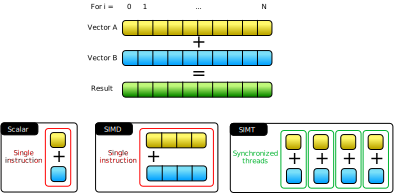
\includegraphics[width=\textwidth]{SIMD_vs_SIMT.png}
    \end{center}
\end{frame}

% _____________________________________________________________________________

\begin{frame}{What's the motivation of putting GPUs in supercomputers?}
    \begin{center}
        \includegraphics[width=0.9\textwidth]{flop_watt_ratio_history_fp64.png}
    \end{center}

    \structure{Question:} How to build the fastest machine with the lowest power consumption and the lowest cost?
\end{frame}

% _____________________________________________________________________________

\begin{frame}{Parallel programming models and libraries in numerical science}
    \begin{center}
        \includegraphics[width=\textwidth]{prog_model.png}
    \end{center}
    \begin{itemize}
        \item Performance portability is one thing
        \item But we will see that developers need more
    \end{itemize}
\end{frame}

% _____________________________________________________________________________

\begin{frame}{Performance, portability and productivity}
    \begin{itemize}
        \item What developers want
        \begin{description}[Interporability]
            \item[Performance] Get the best performance on a specific hardware
            \item[Portability] Run the same code on different hardware
            \item[Productivity] Write code quickly and easily, maintain and extend code, leverage architecture optimization
        \end{description}
        \item What developers for science also want
        \begin{description}[Interporability]
            \item[Maturity] Production-ready (i.e. not research product)
            \item[Community] Contributors, support, documentation, examples
            \item[Longevity] Long-term maintenance, bug fixes, updates, sponsorship
            \item[Interporability] Possibility to easily couple with other libraries and tools (IO, Linear Algebra, Machine leaning, etc.)
        \end{description}
    \end{itemize}
\end{frame}
% _____________________________________________________________________________

\begin{frame}{Do you need performance portability?}
    \begin{itemize}
        \item Probably yes if you...
        \begin{itemize}
            \item Want your code to run on different hardware technologies (CPU, GPU)
            \item Have performance requirements
            \item Cannot afford to maintain and optimize different versions of your code for each possible hardware of the market
            \item Want to focus on algorithmic and not on code development
            \item Want your code to be easily maintainable and readable by others, especially non experts
        \end{itemize}
        \item Maybe not if you...
        \begin{itemize}
            \item Need to tune your algorithms to work as fast as possible on a given hardware
        \end{itemize}
    \end{itemize}
\end{frame}

% _____________________________________________________________________________

\begin{frame}{Kokkos programming model}
    Kokkos is a performance portability parallel programming model build upon the C++-17 standard, designed to abstract already existing parallel programming models

    \vspace{0.5em}

    \begin{itemize}
        \item Kokkos provides data structures and functions based on modern C++ to build your application
        \item Developers never directly use underlying backends (no CUDA kernels for instance)
    \end{itemize}
    \begin{center}
        
\includegraphics[width=1\textwidth]{kokkos_model.png}
    \end{center}
\end{frame}

% _____________________________________________________________________________

\begin{frame}{Kokkos parallelism scope}
    \begin{itemize}
        \item Kokkos only handle node-level parallelism
        \item You still need a model for distributed memory parallelism (e.g. MPI)
    \end{itemize}
\end{frame}

% _____________________________________________________________________________

\begin{frame}{Kokkos: a tool for both C++ beginners and experts}
    \begin{itemize}
        \item Kokkos' basic capabilities
        \begin{itemize}
            \item Abstraction of most parallel patterns used in HPC (loops, reduction, scan)
            \item Abstracted basic data structures used in science (vectors, multidimensional arrays, sub-arrays, strided arrays, etc)
        \end{itemize}
        \item Kokkos' advanced capabilities
        \begin{itemize}
            \item Advanced data structure properties
            \item Thread safety, thread scalability, and atomic operations
            \item Hierarchical patterns for maximizing parallelism
        \end{itemize}
        \item Kokkos' tools and Kernels
        \begin{itemize}
            \item Profiling, tuning and debuging tools
            \item Interacting with Python and Fortran
            \item Library extensions: Kokkos-Kernels for Linear Algebra, Kokkos-FFT, Kokkos-Comm and more
        \end{itemize}
    \end{itemize}
\end{frame}

% _____________________________________________________________________________

\begin{frame}{Kokkos ecosystem}
    \begin{center}
        \includegraphics[width=\textwidth]{kokkos-ecosystem.png}
    \end{center}
\end{frame}

% _____________________________________________________________________________

\begin{frame}{Kokkos and the evolution of the C++ standard}
    \begin{center}
        \includegraphics[width=\textwidth]{kokkos-cpp-standard.png}
    \end{center}
\end{frame}

% _____________________________________________________________________________

\begin{frame}{Kokkos useful resources}
    \begin{itemize}
        \item GitHub repository: \url{https://github.com/kokkos}
        \item Documentation: \url{https://kokkos.org/kokkos-core-wiki}
        \item Cheat sheet: \url{https://github.com/CExA-project/cheat-sheet-for-kokkos/releases/latest}
        \item Slack channel: \url{https://kokkosteam.slack.com}
    \end{itemize}
\end{frame}

% _____________________________________________________________________________

\section{Basic concepts of Kokkos}

% _____________________________________________________________________________

\subsection{Compilation}

% _____________________________________________________________________________

\begin{frame}{Compiling Kokkos from source}
    \begin{itemize}
        \item Require CMake and a C++ compiler
        \item Compile Kokkos as an external library or as part of your project (inline build) using the source
        \item You can use Spack to install Kokkos
        \item You can get the source code from the \href{https://github.com/kokkos/kokkos}{Kokkos GitHub repository}
    \end{itemize}
    \begin{center}
        \includegraphics[width=0.15\textwidth]{spack.png}
        \includegraphics[width=0.15\textwidth]{GitHub-logo.png}
    \end{center}
\end{frame}

% _____________________________________________________________________________

\begin{frame}{The notion of backend in Kokkos}
    \begin{itemize}
        \item Kokkos is compiled to target a specific backend
        \item Only one CPU backend and one GPU backend maximum can be compiled at a time
        \item Kokkos is portable until you compile it. You need one compilation per backend
    \end{itemize}
    \begin{center}
        
\includegraphics[width=0.6\textwidth]{kokkos_backend.png}
    \end{center}
\end{frame}

% _____________________________________________________________________________

\begin{frame}[fragile]{Compiling Kokkos with the default parameters}
    \begin{itemize}
        \item Install Kokkos with the serial backend
        \item Use the default compiler or specify it with \texttt{-DCMAKE\_CXX\_COMPILER}
    \end{itemize}
    \begin{minted}{bash}
cmake ${srcdir} \
    -DCMAKE_CXX_COMPILER=g++ \
    -DCMAKE_INSTALL_PREFIX=${kokkos_install_folder}
    \end{minted}
\end{frame}

% _____________________________________________________________________________

\begin{frame}[fragile]{Compiling Kokkos for a specific backend}
    \begin{itemize}
        \item Add the CMake option \texttt{-DKokkos\_ENABLE\_<BACKEND>=ON} to enable a specific backend, replacing \texttt{<BACKEND>} with the backend name
        \item Serial backend is \texttt{SERIAL}
        \item CPU backends are \texttt{OPENMP}, \texttt{THREADS}, \texttt{HPX}
        \item GPU backends are \texttt{CUDA}, \texttt{HIP}, \texttt{SYCL}
    \end{itemize}
    \begin{minted}[texcomments]{bash}
cmake ${srcdir} \
    -DCMAKE_CXX_COMPILER=g++ \
    -DCMAKE_INSTALL_PREFIX=${kokkos_install_folder} \
    -DKokkos_ENABLE_CUDA=ON
    \end{minted}
\end{frame}

% _____________________________________________________________________________

\begin{frame}{Warning regarding the Kokkos compilation}
    \begin{itemize}
        \item All backends \highlight{do not have the same level of maturity}, some are experimental!
        \item The backend environment (for instance CUDA) must be available on the target machine, \highlight{Kokkos does not install it for you}!
    \end{itemize}
\end{frame}

% _____________________________________________________________________________

\begin{frame}{Compiling Kokkos for a specific archiecture}
    \begin{itemize}
        \item Architecture CMake options \texttt{-DKokkos\_ARCH\_<ARCH\_NAME>=ON} can be specified for best performance
        \item Replace \texttt{<ARCH\_NAME>} with the architecture name of the target host and device
        \item For example, for a NVIDIA A100 GPU, the architecture name is \texttt{AMPERE80}
        \item All CMake options are available \href{https://kokkos.org/kokkos-core-wiki/keywords.html}{on the dedicated doc page}
    \end{itemize}
\end{frame}

% _____________________________________________________________________________

\begin{frame}[fragile]{Compiling for a multi-core Xeon Skylake CPU and a A100 NVIDIA GPU}
    \begin{itemize}
        \item OpenMP option for the multi-core CPU
        \item Skylake option, mostly for vectorization (optional)
        \item CUDA option for the GPU
        \item A100 option, for the correct architecture (mandatory)
    \end{itemize}
    \begin{minted}{bash}
cmake ${srcdir} -DCMAKE_INSTALL_PREFIX=${kokkos_install_folder} \
    -DKokkos_ENABLE_OPENMP=ON \
    -DKokkos_ARCH_SKX=ON \
    -DKokkos_ENABLE_CUDA=ON \
    -DKokkos_ARCH_AMPERE80=ON
    \end{minted}
    \begin{center}
        \includegraphics[width=0.5\textwidth]{kokkos_a100_backend.png}
    \end{center}
\end{frame}
% _____________________________________________________________________________

\begin{frame}{Exercise 1: learn how to compile Kokkos}
    \begin{center}
    
\includegraphics[width=0.4\textwidth]{sleeping_otter.png}
    \end{center}

    Go to the folder \href{https://github.com/CExA-project/cexa-kokkos-tutorials/tree/main/exercises/01_compiling_kokkos}{01\_compiling\_kokkos} and follow the instructions in the README file

    \begin{block}{Goals of this exercise}
        \begin{itemize}
            \item Compile Kokkos with the default parameters
            \item Compile Kokkos with the OpenMP backend
            \item Compile Kokkos with a GPU backend
        \end{itemize}
    \end{block}
\end{frame}

% _____________________________________________________________________________

\subsection[Starting a Kokkos program]{Starting and compiling a Kokkos program}

% _____________________________________________________________________________

\begin{frame}[fragile]{Start a Kokkos program}
    \begin{itemize}
        \item Include the Kokkos header file (like any other library)
        \item Use the Kokkos namespace \texttt{Kokkos::}
        \item Initialize and finalize Kokkos (like MPI)
    \end{itemize}
    \begin{minted}{C++}
#include <Kokkos_Core.hpp>

int main(int argc, char* argv[]) {
    Kokkos::initialize(argc, argv);
    {
        // Your code here
    }
    Kokkos::finalize();
}
    \end{minted}
\end{frame}

% _____________________________________________________________________________

\begin{frame}[fragile]{ScopeGuard: an alternative to initialize and finalize}
    \begin{itemize}
        \item \texttt{ScopeGuard} is a class that ensure that \texttt{Kokkos::initialize} and \texttt{Kokkos::finalize} are called correctly
        \item Resource Acquisition Is Initialization (RAII) pattern
    \end{itemize}
    \begin{minted}{C++}
#include <Kokkos_Core.hpp>

int main(int argc, char* argv[]) {
    Kokkos::ScopeGuard guard(argc, argv);

    // Your code here
}
    \end{minted}
\end{frame}

% _____________________________________________________________________________

\begin{frame}[fragile]{Use CMake to compile your Kokkos program}
    \begin{itemize}
        \item Kokkos should be compiled and installed on your system
        \item Use the \texttt{find\_package} CMake command to find Kokkos
        \item Use the \texttt{target\_link\_libraries} CMake command to link your program with Kokkos
    \end{itemize}
    \begin{minted}{cmake}
cmake_minimum_required(VERSION 3.16)
project(my_kokkos_project LANGUAGES CXX)
find_package(Kokkos REQUIRED)
add_executable(test main.cpp)
target_link_libraries(test Kokkos::kokkos)
    \end{minted}
\end{frame}

% _____________________________________________________________________________

\begin{frame}[fragile]{Use CMake to compile your Kokkos program}
    \begin{itemize}
        \item Kokkos propagates its compilation flags to your program
        \item If Kokkos is not detected in your paths, use the \texttt{Kokkos\_ROOT} CMake variable to specify the path to Kokkos
    \end{itemize}
    \begin{minted}{bash}
cmake ${srcdir} \
  -DKokkos_ROOT=${kokkos_install_prefix} \
  -DCMAKE_CXX_COMPILER=${compiler_used_to_build_kokkos}
    \end{minted}
\end{frame}

% _____________________________________________________________________________

\begin{frame}[fragile]{Exercise 2: learn how to compile a Kokkos program}
    \begin{center}
        
\includegraphics[width=0.4\textwidth]{sleeping_otter.png}
    \end{center}

    Go to the folder \href{https://github.com/CExA-project/cexa-kokkos-tutorials/tree/main/exercises/02_first_program}{02\_first\_program} and follow the instructions in the README file

    \begin{block}{Goals of this exercise}
        \begin{itemize}
            \item Write a simple Kokkos program
            \item Compile the program with CMake
        \end{itemize}
    \end{block}
\end{frame}

% _____________________________________________________________________________

\subsection[Data container]{Data container}

% _____________________________________________________________________________

\begin{frame}[fragile]{Kokkos' abstracted data container}
    \begin{itemize}
        \item Why is it important to have an abstracted data container?
        \begin{itemize}
            \item No need to allocate or deallocate memory by hand
            \item Vendor-specific memory allocation is hidden
            \item Unified semantic and portable memory management (CPU and GPU)
            \item Advanced capability (abstracted layout, subarray, multidimensionality, etc.)
        \end{itemize}
        \item Kokkos provides the View class
        \begin{itemize}
            \item View is an abstraction of the notion of vector (resize function for instance) and multidimensional array
            \item Bring portable Python numpy/Fortran-like syntax for multidimensional arrays
        \end{itemize}
    \end{itemize}
\end{frame}

% _____________________________________________________________________________

\begin{frame}[fragile]{Creating a View}
    \begin{itemize}
        \item View is a template class
        \item Contains any C++ type (\texttt{int}, \texttt{float}, \texttt{double}, etc)
        \item Number of dimensions fixed at compilation time
        \item Size of each dimension determined at compilation time or runtime
    \end{itemize}
    \begin{minted}{C++}
Kokkos::View<int[10]> view1 ("my view of static size");
Kokkos::View<float*> view2 ("my view of dynamic size", 10);
Kokkos::View<double*[10]> view3 (
        "my view of static and dynamic size", 10);
    \end{minted}
\end{frame}

% _____________________________________________________________________________

\begin{frame}[fragile]{Accessing the data}
    \begin{itemize}
        \item Data are accessed using the parenthesis operator \texttt{(i, j, k, ...)}
        \item Raw data can be accessed using the \texttt{data()} method (not recommended)
    \end{itemize}
    \begin{minted}{C++}
const int Nx = 1000;
const int Ny = 2000;

Kokkos::View<int**> my_matrix("matrix", Nx, Ny);

for (int i = 0; i < Nx; i++) {
    for (int j = 0; j < Ny; j++) {
        my_matrix(i,j) = i + j;
    }
}
    \end{minted}
\end{frame}

% _____________________________________________________________________________

\begin{frame}{Where does the data reside?}
    \begin{itemize}
        \item A View lives in a specific memory space (Host or Device), not both
        \item If Kokkos is compiled with a \highlight{CPU backend only}, the View data is allocated in the \highlight{Host memory} by default
    \end{itemize}
    \begin{center}
        \includegraphics[width=0.7\textwidth]{host_view_memory.png}
    \end{center}
\end{frame}

% _____________________________________________________________________________

\begin{frame}{Where does the data reside?}
    \begin{itemize}
        \item If Kokkos is compiled with a \highlight{GPU backend}, the View data is allocated in the \highlight{Device memory} by default
        \item Device view data \highlight{cannot} be accessed on the Host and vice versa
        \item We will later see how to allocate and copy data between the Host and the Device
    \end{itemize}
    \begin{center}
        \includegraphics[width=0.7\textwidth]{device_view_memory.png}
    \end{center}
\end{frame}

% _____________________________________________________________________________

\begin{frame}{More about dynamic views}
    \begin{itemize}
        \item Allocations only happen when explicitly specified
        \item Copy construction and assignment are shallow: you pass Views by value, not by pointer or reference (unlike C arrays)
        \item Reference counting is used for automatic deallocation (like shared pointers)
        \item Metadata (rank, extent, etc) is however always accessible on the Host
        \item Views have a \highlight{limited} number of dimensions (up to 7)
    \end{itemize}
\end{frame}

% _____________________________________________________________________________

\begin{frame}{Useful methods to manage View}
    \begin{itemize}
        \item \texttt{rank()}: return the rank of the view (number of dimensions)
        \item \texttt{extent(const int dim)}: return the size of a specific dimension
        \item \texttt{size()}: return the total number of elements
        \item many others but not the subject of this introduction
    \end{itemize}
\end{frame}

% _____________________________________________________________________________

\begin{frame}{Notion of View layout}
    \begin{itemize}
        \item Layout is the way to map multidimensional index to memory
        \item Kokkos provides an abstraction of the data layout
        \item The default layout of a View depends on the backend (Host or Device)
        \item How to manipulate the layout is not the subject of this introduction
    \end{itemize}
    \begin{center}
        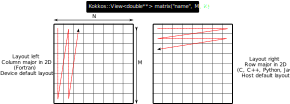
\includegraphics[width=0.95\textwidth]{layout_right_left.png}
    \end{center}
\end{frame}

% _____________________________________________________________________________

\begin{frame}{Exercise 3: learn how to use a View}
    \begin{center}
        
\includegraphics[width=0.4\textwidth]{sleeping_otter.png}
    \end{center}

    Go to the exercise \href{https://github.com/CExA-project/cexa-kokkos-tutorials/tree/main/exercises/03_basic_view}{03\_basic\_view} and follow the instructions in the README file

    \begin{block}{Goals of this exercise}
        \begin{itemize}
            \item Create and manage a View
        \end{itemize}
    \end{block}
\end{frame}

% _____________________________________________________________________________

\begin{frame}{Understand the notion of memory space}
    \begin{itemize}
        \item Kokkos provides an abstraction of where the data lives: the \highlight{memory space}
        \item A View is always associated with a defined memory space (Host or Device for instance) at compilation time
        \item By default, view data is allocated in the Host memory space if no GPU backend is available, otherwise in the Device memory space
    \end{itemize}
\end{frame}

% _____________________________________________________________________________

\begin{frame}{Understand the notion of memory space}
    \structure{Problem:} How to deal with data living in different memory spaces?

    \begin{center}
        \includegraphics[width=\textwidth]{device_memory_access.png}
    \end{center}

\end{frame}

% _____________________________________________________________________________

\begin{frame}[fragile]{Understand the notion of memory space}
    A template argument \texttt{MemorySpace} is used to specify the memory space when creating a view

    \begin{minted}{C++}
Kokkos::View<int**, MemorySpace> my_matrix("matrix", Nx, Ny);
    \end{minted}
    \begin{itemize}
        \item Host space is \texttt{Kokkos::HostSpace}
        \item Beginners usually does not set the memory space
        \item Using a vendor-specific memory space breaks the portability of the code
    \end{itemize}
\end{frame}

% _____________________________________________________________________________

\begin{frame}[fragile]{Mirror Views presentation}
    \structure{Solution:} We need to connect host and device views to access data on both sides
    \begin{itemize}
        \item Kokkos provides the notion of \highlight{mirror views}
        \item A mirror view is similar to its original view but lives in a different memory space
        \item A mirror view automatically inherits the properties of the original view (extent, layout, etc)
        \item There is a specific function to create a mirror view called \texttt{create\_mirror}
        \item It can be used to create a host mirror of a device view
    \end{itemize}
    \begin{minted}{C++}
Kokkos::View<int**> device_matrix("device_matrix", Nx, Ny);
Kokkos::View<int**>::HostMirror host_matrix =
    Kokkos::create_mirror(device_matrix);
    \end{minted}
\end{frame}

% _____________________________________________________________________________

\begin{frame}{Undestanding mirror View with a device View}
    \begin{center}
        \includegraphics[width=\textwidth]{device_mirror_view.png}
    \end{center}
\end{frame}

% _____________________________________________________________________________

\begin{frame}{Views and mirror Views in the host memory space}
    \begin{itemize}
        \item For portability reason, we always use a mirror view whether we compile with a CPU or GPU backend
        \item With a CPU backend only, the mirror view lives in the same memory space as the original view
    \end{itemize}

    \structure{Problem:} The \texttt{create\_mirror} function always create a view with allocated memory (i.e. memory duplication)

    \begin{center}
        \includegraphics[width=0.9\textwidth]{host_mirror_view.png}
    \end{center}
\end{frame}

% _____________________________________________________________________________

\begin{frame}{Views and mirror Views in the host memory space}
    \structure{Solution:} Use \texttt{create\_mirror\_view}

    \begin{itemize}
        \item The function \texttt{create\_mirror\_view} is used to create a mirror without allocating memory if the mirror view lives in the same memory space as the original view
        \item The new view is a shallow copy of the original view (i.e. it targets the same data)
    \end{itemize}
    \begin{center}
        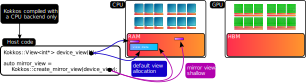
\includegraphics[width=0.9\textwidth]{host_create_mirror_view.png}
    \end{center}
\end{frame}

% _____________________________________________________________________________

\begin{frame}[fragile]{Deep copy function to exchange data between memory spaces}
    \begin{itemize}
        \item Kokkos provides a function \texttt{deep\_copy} to copy data between views in different memory spaces
        \item Views must have the same layout and extent
        \item The function is used to copy data from the source view to the destination view
        \item If the destination view is a shallow copy of the source view (e.g. \texttt{create\_mirror\_view} on Host), the function does nothing (portability)
    \end{itemize}
    \begin{minted}{C++}
Kokkos::deep_copy(destination, source);
    \end{minted}
\end{frame}

% _____________________________________________________________________________

\begin{frame}[fragile]{Deep copy example between Host and Device}
    \begin{minted}{C++}
Kokkos::View<int**> device_matrix("device_matrix", Nx, Ny);

Kokkos::View<int**>::HostMirror host_matrix =
    Kokkos::create_mirror(device_matrix);

Kokkos::deep_copy(device_matrix, host_matrix);
    \end{minted}
\end{frame}

% _____________________________________________________________________________

\begin{frame}{Deep copy function to exchange data between memory spaces}
    \begin{center}
        \includegraphics[width=0.9\textwidth]{device_host_deep_copy.png}
    \end{center}
\end{frame}

% _____________________________________________________________________________

\begin{frame}{Exercise 4: Mirror Views and deep copy}
    \begin{center}
        
\includegraphics[width=0.4\textwidth]{sleeping_otter.png}
    \end{center}

    Go to the exercise \href{https://github.com/CExA-project/cexa-kokkos-tutorials/tree/main/exercises/04_deep_copy}{04\_deep\_copy} and follow the instructions in the README file

    \begin{block}{Goal of this exercise}
        \begin{itemize}
            \item Create and manage a mirror view
            \item Use the deep copy function
        \end{itemize}
    \end{block}
\end{frame}

% _____________________________________________________________________________

\subsection{Parallel loops}

% _____________________________________________________________________________

\begin{frame}[fragile]{Kokkos uses the concept of data parallelism as OpenMP}
    \begin{minted}[texcomments]{C++}
for (int i = 0; i < N; i++) {
    A(i) = B(i) + C(i) * D(i);
}
    \end{minted}
    \begin{itemize}
        \item \textcolor{gray}{\texttt{for}} is the loop pattern (for, reduction, scan, graph)
        \item \textcolor{gray}{\texttt{int i = 0; i < N; i++}} is the execution policy
        \item \textcolor{gray}{\texttt{A(i) = B(i) + C(i) * D(i)}} is the kernel
    \end{itemize}
\end{frame}

% _____________________________________________________________________________

\begin{frame}[fragile]{Simple parallel loop with Kokkos and OpenMP}
    FMA addition using a parallel loop

    \begin{itemize}
        \item Kokkos version
        \begin{minted}{C++}
Kokkos::parallel_for("my_loop", N,
KOKKOS_LAMBDA(int i) {
    A(i) = B(i) + C(i) * D(i);
});
        \end{minted}
        \item OpenMP version
        \begin{minted}{C++}
#pragma omp parallel for
for (int i = 0; i < N; i++) {
    A(i) = B(i) + C(i) * D(i);
});
        \end{minted}
    \end{itemize}
\end{frame}

% _____________________________________________________________________________

\begin{frame}[fragile]{Simple parallel loop with Kokkos explained}
    \begin{itemize}
        \item \textcolor{gray}{\texttt{Kokkos::parallel\_for}} is the loop pattern
        \item \textcolor{gray}{\texttt{N}} and \texttt{int i} is the execution policy (can't be simpler)
        \item \textcolor{gray}{\texttt{KOKKOS\_LAMBDA(int i) \{A(i) = B(i) + C(i) * D(i)\}}} is the kernel
    \end{itemize}
    \begin{minted}{C++}
Kokkos::parallel_for("my_loop", N,
KOKKOS_LAMBDA(int i) {
    A(i) = B(i) + C(i) * D(i);
});
    \end{minted}
    \begin{itemize}
        \item The previous OpenMP version only works on CPUs (need \texttt{target} directive for GPUs)
        \item The same Kokkos version works on CPUs and GPUs depending on the compile backend
    \end{itemize}
\end{frame}

% _____________________________________________________________________________

\begin{frame}[fragile]{Notion of C++ Lambda}
    \begin{itemize}
        \item A lambda is a C++ anonymous function, i.e. a function as an object
        \item \texttt{KOKKOS\_LAMBDA} is a macro that creates a lambda function with the correct signature for you
        \item For beginners, no need to understand C++ lambdas to use Kokkos
    \end{itemize}
    \begin{minted}{C++}
Kokkos::parallel_for("my_loop", N,
KOKKOS_LAMBDA(int i) {
    A(i) = B(i) + C(i) * D(i);
});
    \end{minted}
\end{frame}

% _____________________________________________________________________________

\begin{frame}{Where is my parallel loop executed?}
    \begin{itemize}
        \item Where the loop is executed is called the \textcolor{orange}{\textbf{execution space}}
        \item If Kokkos is compiled with a GPU backend, the loop is executed on GPU by default
        \item Otherwise, the loop is executed on the CPU
        \item Non-kokkos C++ code is always executed on the Host
        \item Kokkos loops have a name for debugging purpose
    \end{itemize}
\end{frame}

% _____________________________________________________________________________

\begin{frame}[fragile]{Asynchronous execution}
    \begin{minted}{C++}
// Kokkos parallel loop
Kokkos::parallel_for("my_amazing_loop", N,
    KOKKOS_LAMBDA(int i) { data(i) = ... });

// Host code
amazing_function(data);
    \end{minted}
    \begin{itemize}
        \item If Kokkos uses a GPU backend, the parallel loop is executed asynchronously on the GPU
        \item This mean that the loop is launched and the program continues
        \item Asynchronism is a complex concept for beginners, not the subject of this introduction
    \end{itemize}

    \structure{Problem:} What if I need the results of the parallel loop in the host code?
\end{frame}

% _____________________________________________________________________________

\begin{frame}[fragile]{Fence}
    \structure{Solution:} To make sure that the loop is finished, a \texttt{fence} function is used (equivalent of an OpenMP barrier or a MPI wait)

    \begin{minted}{C++}
// Kokkos parallel loop
Kokkos::parallel_for("my_amazing_loop", N,
    KOKKOS_LAMBDA(int i) { data(i) = ... });

Kokkos::fence("my_amazyng_loop fence");

// Host code
amazing_function(data);
    \end{minted}
\end{frame}

% _____________________________________________________________________________

\begin{frame}{Exercise 5: My first parallel loop}
    \begin{center}
        
\includegraphics[width=0.4\textwidth]{sleeping_otter.png}
    \end{center}

    Go to the exercise \href{https://github.com/CExA-project/cexa-kokkos-tutorials/tree/main/exercises/05_parallel_loop}{05\_parallel\_loop} and follow the instructions in the README file

    \begin{block}{Goal of this exercise}
        \begin{itemize}
            \item Write a simple parallel loop
        \end{itemize}
    \end{block}
\end{frame}

% _____________________________________________________________________________

\subsection[Extended loop policy]{How to extent the loop policy}

% _____________________________________________________________________________

\begin{frame}[fragile]{How to extent the loop policy ?}
    Kokkos provides a way to set how a loop is executed with \highlight{execution policies}

    \begin{minted}{C++}
Kokkos::RangePolicy<ExecutionSpace> policy(start_index, end_index);
    \end{minted}
    \begin{itemize}
        \item \texttt{ExecutionSpace} is an optional template parameter that specifies the execution space, by default the execution space is \texttt{DefaultExecutionSpace}
        \item \texttt{start\_index} and \texttt{end\_index} are the beginning and the end of the loop
    \end{itemize}
\end{frame}

% _____________________________________________________________________________

\begin{frame}[fragile]{How to extent the loop policy ?}
    The following parallel loops are therefore equivalent:

    \begin{minted}{C++}
// Shortcut version
Kokkos::parallel_for("my_loop",
    N,
    KOKKOS_LAMBDA(int i) { ... });
    \end{minted}
    \begin{minted}{C++}
// explicitly specify the execution policy
Kokkos::parallel_for("my_loop",
    Kokkos::RangePolicy<Kokkos::DefaultExecutionSpace>(0, N),
    KOKKOS_LAMBDA(int i) { ... });
    \end{minted}
\end{frame}

% _____________________________________________________________________________

\begin{frame}{Execution Space}
    \begin{itemize}
        \item By specifying the execution space, you control where the loop is executed (CPU or GPU)
        \item \texttt{Kokkos::DefaultExecutionSpace} and \texttt{Kokkos::DefaultHostExecutionSpace} are enough for beginners
        \item Other execution spaces are not the subject of this introduction
        \item This way of doing ensures that the code is portable
    \end{itemize}
    \begin{center}
        \begin{tabular}{lll}
            & \multicolumn{2}{l}{Kokkos compiled on} \\
            Execution space & GPU backend & CPU backend \\
            \texttt{Kokkos::DefaultExecutionSpace} & Runs on GPU & Runs on CPU \\
            \texttt{Kokkos::DefaultHostExecutionSpace} & Runs on CPU & Runs on CPU \\
        \end{tabular}
    \end{center}
\end{frame}

% _____________________________________________________________________________

\begin{frame}{Default execution space summary}
    \begin{center}
        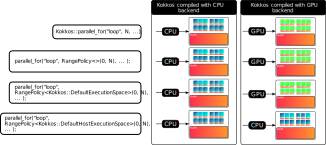
\includegraphics[width=\textwidth]{default_execution_space.png}
    \end{center}
\end{frame}

% _____________________________________________________________________________

\begin{frame}[fragile]{Relation between execution space and memory space}
    The memory space associated with an execution space is retrieved using the \highlight{memory\_space} attribute

    \begin{minted}{C++}
using DefaultMemorySpace =
    Kokkos::DefaultExecutionSpace::memory_space;

using DefaultHostMemorySpace =
    Kokkos::DefaultHostExecutionSpace::memory_space;
// same as Kokkos::HostSpace
    \end{minted}
\end{frame}

% _____________________________________________________________________________

\begin{frame}[fragile]{Nested parallel loops}
    \begin{minted}{C++}
Kokkos::View<int**> my_matrix("matrix", Nx, Ny);

for (int i = 0; i < Nx; i++) {
    for (int j = 0; j < Ny; j++) {
        my_matrix(i,j) = i + j;
    }
}
    \end{minted}
\end{frame}

% _____________________________________________________________________________

\begin{frame}[fragile]{Nested parallel loops}
    \begin{itemize}
        \item Kokkos has a specific execution policy for nested parallel loops
        \item The \texttt{MDRangePolicy} (with \emph{MD} for multidimensional)
        \item Somehow similar to the \texttt{collapse} directive in OpenMP
        \item Addition of the \texttt{Rank} template parameter to specify the dimensions
    \end{itemize}
    \begin{minted}{C++}
Kokkos::MDRangePolicy<
    ExecutionSpace,
    Kokkos::Rank<2>> policy(
        {start_index_i, start_index_j},
        {end_index_i, end_index_j});
    \end{minted}
\end{frame}

% _____________________________________________________________________________

\begin{frame}[fragile]{Nested parallel loops in practice}
    \begin{minted}{C++}
Kokkos::View<int**> my_matrix("matrix", Nx, Ny);

Kokkos::parallel_for("my_loop",
    Kokkos::MDRangePolicy<ExecutionSpace, Kokkos::Rank<2>>(
        {0, 0}, {Nx, Ny}),
    KOKKOS_LAMBDA(int i, int j) {
        my_matrix(i, j) = i + j;
    }
);
    \end{minted}
\end{frame}

% _____________________________________________________________________________

\subsection[Parallel reduction]{Parallel reduction}

% _____________________________________________________________________________

\begin{frame}[fragile]{Parallel reduction}
    \begin{itemize}
        \item Parallel reduction is the second loop pattern provided by Kokkos: \texttt{Kokkos::parallel\_reduce}
        \item It is used to compute a single value from an array (sum, max, min, etc.)
        \item It works like the \texttt{parallel\_for} loop pattern with an additional argument: the reducer operation to perform \texttt{Kokkos::Reducer\_op<type>}
        \item \texttt{KOKKOS\_LAMBDA} also has an additional argument: a reference to the local result
    \end{itemize}
    \begin{minted}{C++}
// No need to initialize the output variable, it will be
// done by the parallel_reduce call
double result;

Kokkos::parallel_reduce("my_reduction", N,
    KOKKOS_LAMBDA(int i, double& local_result) {
        local_result += i;
    }, Kokkos::Sum<double>(result));
    \end{minted}
\end{frame}

% _____________________________________________________________________________

\begin{frame}{Parallel reduction explained}
    \begin{itemize}
        \item Works like \texttt{parallel\_for} (e.g. execution space)
        \item Reduction is always optimized for the selected execution space
        \item Kokkos provides various reducers (\texttt{Reducer\_op}) for the most common operations:
        \begin{itemize}
            \item \texttt{Kokkos::Sum}: Sum of the elements
            \item \texttt{Kokkos::Max}: and \texttt{Kokkos::Min}: Maximum and minimum element
            \item \texttt{Kokkos::Prod}: Product of the elements
            \item \texttt{Kokkos::MaxLoc} and \texttt{Kokkos::MinLoc}: Maximum and minimum element with their index
            \item More \href{https://kokkos.org/kokkos-core-wiki/ProgrammingGuide/Custom-Reductions-Built-In-Reducers.html}{in the doc}
        \end{itemize}
        \item You can also create your own reducer but this is not the subject of this introduction
    \end{itemize}
\end{frame}

% _____________________________________________________________________________

\begin{frame}[fragile]{Sum reduction example}
    \begin{minted}{C++}
Kokkos::View<double*> A("A", N);
// Fill vector A with data

double result;
Kokkos::parallel_reduce("my_reduction", N,
    KOKKOS_LAMBDA(int i, double& local_result) {
        local_result += A(i);
    }, Kokkos::Sum<double>(result)); // or just `result` for sum
    \end{minted}
\end{frame}

% _____________________________________________________________________________

\begin{frame}[fragile]{Max reduction example}
    \begin{minted}{C++}
Kokkos::View<double*> A("A", N);
// Fill vector A with data

double max_value;
Kokkos::parallel_reduce("my_reduction", N,
    KOKKOS_LAMBDA(int i, double& local_max_value) {
        local_max_value = Kokkos::max(A(i), local_max_value);
    }, Kokkos::Max<double>(max_value));
    \end{minted}
\end{frame}

% _____________________________________________________________________________

\begin{frame}[fragile]{Min and index reduction example}
    \begin{minted}{C++}
Kokkos::View<double*> A("A", N);
// Fill vector A with data

// Use a structure containing val and loc variables
using minloc_type = Kokkos::MinLoc<double, int>::value_type;

minloc_type minloc;
Kokkos::parallel_reduce( "MinLocReduce", N,
    KOKKOS_LAMBDA (int i, minloc_type& lminloc) {
        if (A(i) < lminloc.val) {
            lminloc.val = A(i);
            lminloc.loc = i;
        }
    }, Kokkos::MinLoc<double, int>(minloc));
    \end{minted}
\end{frame}

% _____________________________________________________________________________

\begin{frame}{Exercise 6: Parallel Reduction}
    \begin{center}
        
\includegraphics[width=0.4\textwidth]{sleeping_otter.png}
    \end{center}

    Go to the exercise \href{https://github.com/CExA-project/cexa-kokkos-tutorials/tree/main/exercises/06_parallel_reduce}{06\_parallel\_reduce} and follow the instructions in the README file

    \begin{block}{Goal of this exercise}
        \begin{itemize}
            \item Perform a parallel reduction
        \end{itemize}
    \end{block}
\end{frame}

% _____________________________________________________________________________

\section[Conclusion]{Conclusion}

% _____________________________________________________________________________

\begin{frame}{Conclusion}
    Congratulation, you have learned the basics of Kokkos!

    \begin{itemize}
        \item How to compile Kokkos
        \item How to create and manage a simple View
        \item How to use mirror views and deep copy
        \item How to write a parallel loop
        \item How to extend the loop policy
        \item How to use nested parallel loops
        \item How to write a parallel reduction
    \end{itemize}
\end{frame}

\end{document}